\documentclass{tufte-book}

\hypersetup{colorlinks}% uncomment this line if you prefer colored hyperlinks (e.g., for onscreen viewing)

%%
% Book metadata
\title{Hypercompression}
\author{Charles Holbrow}
%\publisher{Publisher of This Book}

%%
% If they're installed, use Bergamo and Chantilly from www.fontsite.com.
% They're clones of Bembo and Gill Sans, respectively.
%\IfFileExists{bergamo.sty}{\usepackage[osf]{bergamo}}{}% Bembo
%\IfFileExists{chantill.sty}{\usepackage{chantill}}{}% Gill Sans

%\usepackage{microtype}

%%
% Symbol for Euro Currency
\usepackage[official]{eurosym}

%%
% For nicely typeset tabular material
\usepackage{booktabs}

%%
% For graphics / images
\usepackage{graphicx}
\setkeys{Gin}{width=\linewidth,totalheight=\textheight,keepaspectratio}
\graphicspath{{graphics/}}

% The fancyvrb package lets us customize the formatting of verbatim
% environments.  We use a slightly smaller font.
\usepackage{fancyvrb}
\fvset{fontsize=\normalsize}

%%
% Prints a trailing space in a smart way.
\usepackage{xspace}

% Inserts a blank page
\newcommand{\blankpage}{\newpage\hbox{}\thispagestyle{empty}\newpage}

\usepackage{units}
% Control the formatting of lists
\usepackage{enumitem}

% Typesets the font size, leading, and measure in the form of 10/12x26 pc.
\newcommand{\measure}[3]{#1/#2$\times$\unit[#3]{pc}}

% Macros for typesetting the documentation
\newcommand{\hlred}[1]{\textcolor{Maroon}{#1}}% prints in red
\newcommand{\hangleft}[1]{\makebox[0pt][r]{#1}}
\newcommand{\hairsp}{\hspace{1pt}}% hair space
\newcommand{\hquad}{\hskip0.5em\relax}% half quad space
\newcommand{\TODO}[1]{\textcolor{red}{\bf TODO:#1}\xspace}
\newcommand{\ie}{\textit{i.\hairsp{}e.}\xspace}
\newcommand{\eg}{\textit{e.\hairsp{}g.}\xspace}
\newcommand{\na}{\quad--}% used in tables for N/A cells

% Title of my thesis project

\newcommand{\thesis}{Hypercompression\xspace}

\begin{document}

% Front matter
\frontmatter

% Full title page
\maketitle

% Contents
\tableofcontents

% Start the main matter (normal chapters)
\mainmatter

% Introduction
\cleardoublepage
\chapter{Introduction}
\label{ch:introduction}

\begin{fullwidth}
  \newthought{At the Media Lab}, we celebrate the study and practice
  of projects that exist outside of established academic
  disciplines. The Media Lab, and the media have described this
  approach as interdisciplinary, cross-disciplinary,
  anti-disciplinary, or post-disciplinary - emphasizing the clich\'{e}
  that traditional academics must become experts in their field, and
  while narrowing their focus, they learn \textit{more and more about
    less and less}, and eventually know \textit{everything about
    nothing}.  \thesis is truly a Media Lab project. It documents the
  creative process throughout the design, development, and performance of
  a new type of audio signal processor. In doing so, it draws from
  music, mathematics, computer science, acoustics, audio engineering
  and mixing, sound reinforcement, multimedia production, and live
  performance.

\end{fullwidth}

\paragraph{Breadth and Depth} How can we describe a project with such
broad subject material?  A natural tension exists between breadth and
depth: Where the \textit{depth} of a strictly disciplinary approach
provides language and abstractions that enable us to describe content
and communicate at a high level, the \textit{breadth} of the
anti-disciplinary approach invites us to partner with collaborators
with diverse backgrounds and abilities. The challenge is to describe
\thesis so that it is accessible to readers from all disciplines. This
thesis proposes the motivation for documenting media that exists
outside of established disciplines. It proposes a strategy for such
documentation, and employs this strategy by documenting the theory,
implementation, and application of \thesis.

\paragraph{Compression and Hypercompression} A traditional
\marginnote{Be aware of the diference between audio data compression
  and audio dynamic range compression. Data compression is the
  practice of reducing the filesize of digitally encoded audio data. A
  dynamic range compressor is one tool used by audio engineers to
  parametrically manipulate the amplitude of an audio signal. In this
  thesis, \textit{compression} refers to \textit{dynamic range
    compression}.}
dynamic range compressor is one of the most powerful and flexible
tools in the audio engineer's toolkit.  A basic compressor can be
thought of as an automatic volume control that simply reduces the
level of an audio signal when the signal exceeds a threshold. By
carefully adjusting the threshold, the input signals, the reduction
amount, and the rate at which the compressor reacts, a skilled audio
engineer can use compression to increase perceived loudness, improve
intelligibility, augment articulation, smooth a performance, shape
transients, extract ambience, de-ess vocals, balance multiple signals,
and add distortion.\cite{Case2007}

While compression of mono and stereo audio is well documented and
understood,\cite{Giannoulis2012, Blesser1969, Katz2007, Case2007}
surround sound compression is relatively less explored.  \thesis
expands on traditional audio compression model by adding 
spatial control. This design introduces two additional high level
spatial parameters: \textbf{link angle} and \textbf{spread}. These
parameters extend the domain of the traditional compressor to include
surround sound spatial manipulation in addition to dynamics
processing, and unlock new creative possibilities for surround sound
designers.

\paragraph{Performance}
\TODO{Comments about live performance}


\section{Structure}
\label{sec:structure}
\TODO{I'll fill this out more as I progress, but this is basically the
  chapter structure I'm imagining. Building the software likely wont
  have enough content for a whole chapter, so I may merge it with the
  math chapter}
\begin{enumerate}
\item Introduction and  Historical Context % context primes for motivation
\item Motivation
\item Framework for multimedia documentation Approach/Computer Systems
\item Describe the Mathematics 
\item Build the Software
\item Live multimedia performance
\item Concert playback recording. 
\item Conclusion/Educational Implications
\end{enumerate}

\section{Context}
\label{sec:context}

\newthought{The Phillips Pavilion} stands out as an inspiration, a
reference, and a guide for projects that successfully disregard the
conventional disciplinary approach to the creative design process. The
pavilion was a commissioned by Phillips Corporation for the Brussels
World's Fair in 1958.\cite{Zvonare} When the architectural offices of
Le Corbusier received the commission, Le Corbusier replied, saying:
``I will not make a pavilion for you but an Electronic Poem and a
vessel containing the poem; light, color image, rhythm and sound
joined together in an organic synthesis.''\cite{Lopez2011}. Indeed,
the pavilion embodied Le Corbusier's description; the resulting
Gesamtkunstwerk included:\cite{Lombardo1996}
\begin{enumerate}
\item A concrete pavilion, designed by architect and composer Iannis
  Xenakis
\item A tape music composition by Iannis Xenakis, approximately 2
  minutes long, played while the audience transitioned
\item A three channel, 8 minute tape music composition, by French-born
  composer Edgard Var\`{e}se
\item A system for spatialized audio across at least 350 loudspeakers
  distributed throughout the pavilion
\item An assortment of visual effects, designed by Le Corbusier in
  collaboration with Philips art director Louis Kalff
\item video consisting mostly of black and white still images,
  projected on two walls inside the pavilion
\end{enumerate} 


\begin{figure*}[h]
  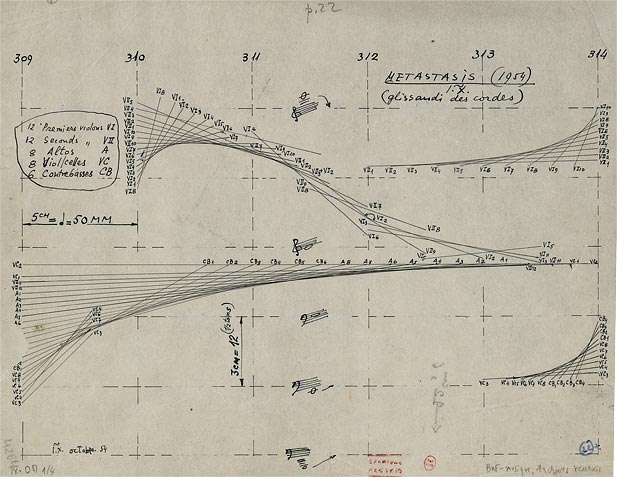
\includegraphics[width=\linewidth]{XenakisMetastasis.jpg}
  \caption{Excerpt from Iannis Xenakis' composition, \textit{Metastasis} (1954)}
  \label{fig:metastasis}
\end{figure*}

\begin{figure*}[h]
  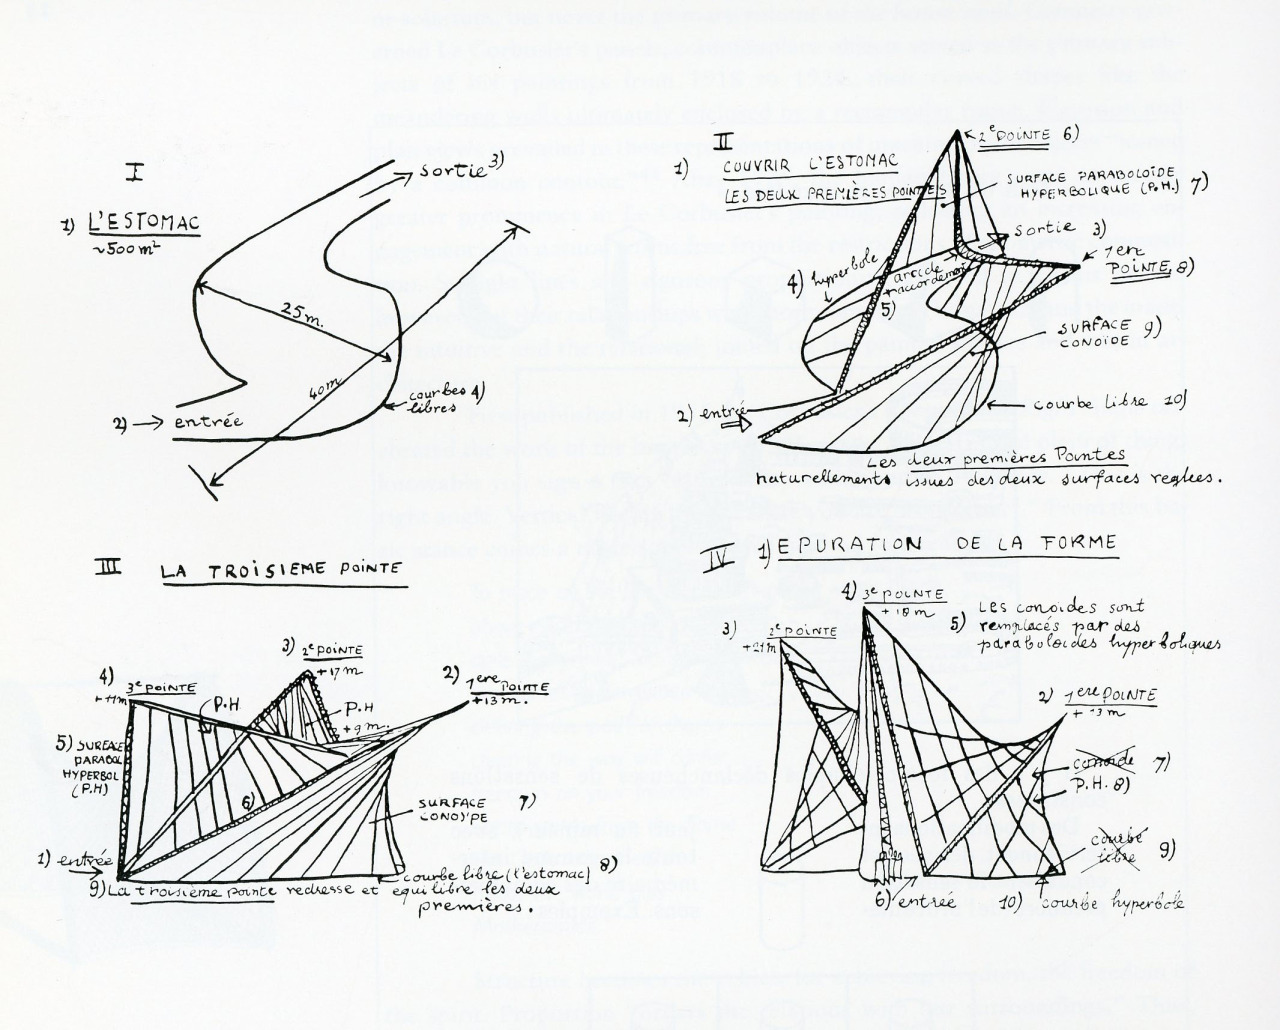
\includegraphics[width=\linewidth]{PhilipsDrawings.jpg}
  \caption{Xenakis' early drawings of the Philips Pavilion as
    documented in the \textit{1958 Philips Technical Review} \TODO{cite}}
  \label{fig:xenakis-draw}
\end{figure*}

\newthought{In 2004}, the Culture 2000 Programme created by the 
European union approved a 99510\EUR{} grant to an Italian Multimedia 
firm for a project called Virtual Electronic Poem (VEP)\cite{eu2004}. 
The project proposed to create a virtual reality simulation in which 
users could experience rendered audio and video of the famous
Gesamtkunstwerk created for the Phillips Pavilion at the 1958 World
Expo in Brussels. 

The goal of the project is included in the Culture 2000 Programme
report: The project will reproduce the experience created by the
Philips pavilion at the Brussels Expo Universelle in 1958.

Give Details? Explain all the parts that were involved with the
original pavilion, explain all the resources that were reviewed to
figure out what the thing actually looked like.

This project was so involved, that the principal investigator coined
the term "Archeology of Multimedia" to describe the experience of
recovering\TODO{cite}.

Virtual reality technology has changed enough between 2004 and 2015,
that reviving the VEP project would probably take an additional
multimedia archeology expedition.

The problem of preservation described above informs the structure and
strategy in this thesis. 

Explain the need for audio systems as computer systems? Cite
Granularity. Describe what fields I draw from. Describe how fields can
go deep, but Anti Disciplinary is unbounded. Describe how this could
only happen at the media lab. Detail how I will granular-ize?

\section{Motivation}
\label{sec:motivation}

  - Sal Khan's talk about students who get stuck. 
  - Talk about the expectations for this paper - what should you
    already understand? Basic Audio theory. 
  - specialization makes it hard for different fields to communicate
  with each other and learn from each other.
  - Think about documentation in terms of Systems, Granulatiry
  - Noticed how very simple concepts are portrayed 
  - Leave behind bridges between disciplines
  - set builder notation, and un-googleable
  questions. IE. Gessamtkunstwerk is googleable, and does not need a
  citation. 

\backmatter

\chapter*{Acknowledgements}
\label{ch:acknowledgements}

\begin{fullwidth}
Thanks to Tod Machover, for your continuous support and encouragement,
for sharing your process, and for help and support integrating \thesis
into \textit{Of Experience}.

Thanks to James Andy Moorer and Joe Paradiso for support, guidance and
mentorship.\TODO{verify spelling}

Thanks to professor Alex Case for the most inspiring my love for
music, audio engineering, and illuminating the magical subtleties of
dynamic range compression.

Thanks to Wonshik Choi and Niyom Lue for your infinite patience,
guidance, and for welcoming me to MIT in 2008. Only you could have
taught a music major to enjoy linux, DSP, and spectroscopy.

Thanks to Shawn Drost for directly and indirectly giving me confidence
as a software developer.

Thanks to my UMass Lowell Piano teachers for taking chance with me,
and putting up with me for four years. Anthony Mele, Elizabeth
Skavish, Bonnie Anderson, and Thomas Stumpf - You believed in me
before I did. I'm probably the only student ever who was lucky enough
to study with all four of you. :P

Thanks to Gene Atwood for being considerate of everyone, and showing
me how important that is -- And for screaming in to a microphone when
I needed some screams.

Thanks to Ben Bloomberg for being my peer and my mentor at the same
time. Thanks for bringing me into the Opera group in 2008 and bringing
me back in 2014. Thanks to Bryn Bliska, for proposing polytempic
modulation, and sharing letting me work out the maths. Thanks to
Rebecca Kleinberger and Akito Van Troyer for your unending support and
encouragement. 

Thanks to Helen Corless for being amazing supportive even when I am in
the absolute pits of grad student existence. Thank you for always
reminding me what music is really about, and for challenging me like
no one else can.

Thanks to my grandparents for leading by example, and teaching
kindness and dedication, and for endless support in education.

Thanks to Hilary, Giles, and Felicity for always inspiring me with
kindness, honesty, and wisdom. 

And thanks to my parents, Gwen and Mark for forcing me to get an
education before I was wise enough to know I wanted one. Thank you for
all your love and support in everything ever I have ever done.
\end{fullwidth}
%%% Local Variables:
%%% mode: latex
%%% TeX-master: t
%%% End:


\bibliography{library}
\bibliographystyle{plainnat}

\end{document}


%%% Local Variables:
%%% mode: latex
%%% TeX-master: t
%%% End:
